\documentclass{report}

\usepackage{graphicx}

\graphicspath{{./assets/}}

\title{SER-210 Final: Design Report}
\author{Thomas Kwashnak}

\begin{document}
\maketitle

\tableofcontents
\newpage

\chapter{Introduction}

\section{About the App}
The app described in this report is an attempt at making an easy go-to chat app to communicate with team members when working on a Github account. It aims to provide quick and easy chat rooms for each repositoriy, while only requiring the user to have a Github account.

\section{Report Purpose}
The purpose of this report is to provide an outline of plans made for the creation of the app. This report contains the UI Design plans, System Design plans, as well as an overview on the production plan over 3 iterations.

\section{User Stories}
\textit{Last Modified: 4/13/2022}
\begin{itemize}
    \item As a user, I can sign in with my GitHub account to sign into the app
    \item As a user, I can view a list of recent chat rooms to quickly get back to what I was working on
    \item As a user, I can tap a star on a chat room to pin it to the top of the list so I have easy access to chat rooms I want
    \item As a user, I can select a chat room to open it up
    \item As a user, I can type and send a message into the chat room to interact with the conversation
    \item As a user, I can see chat messages appear so I can keep up with the conversation
    \item As a user, I can share a chat so I can invite friends into the chat
    \item As a user, I can create a new chat room for a repository that I own so I can coordinate with other contributors
    \item As a user, I can type \# to reference a pull request or issue so they appear in chat as a clickable item
\end{itemize}

\chapter{UI Design}

\section{Navigation Map}
\begin{center}
    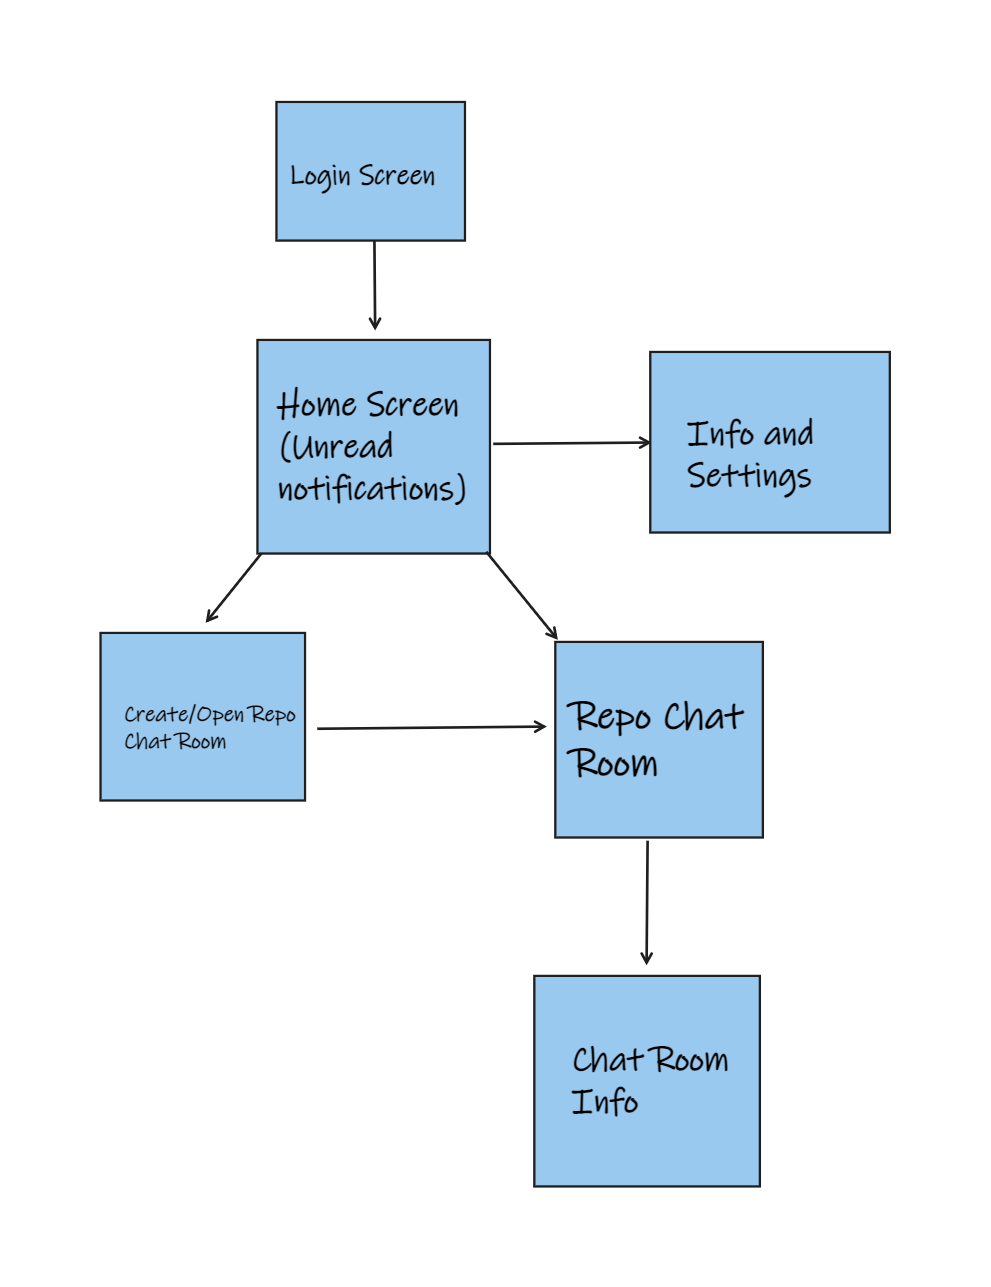
\includegraphics[width=\textwidth]{nav-graph}
\end{center}


\section{App Wireframes}

\newpage
\subsection{Login Page}

\begin{center}
    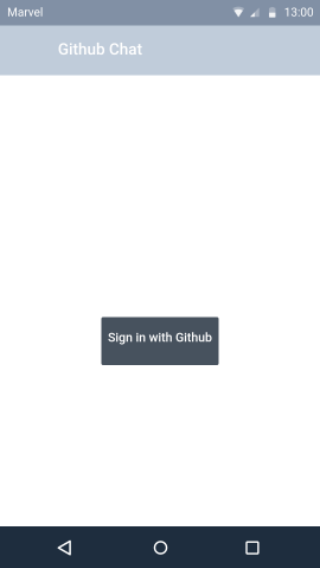
\includegraphics[scale=0.6]{design-login}
\end{center}

\newpage
\subsection{Home Screen}

\begin{center}
    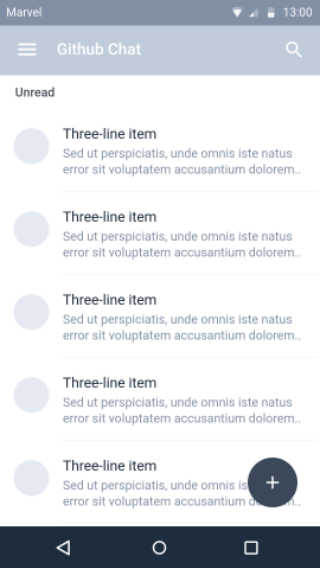
\includegraphics[scale=0.6]{design-home}
\end{center}

\newpage
\subsection{Navigation Drawer}

\begin{center}
    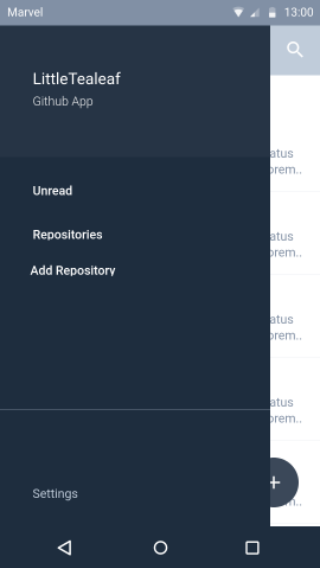
\includegraphics[scale=0.6]{design-nav-drawer}
\end{center}

\newpage
\subsection{Options Screen}
\begin{center}
    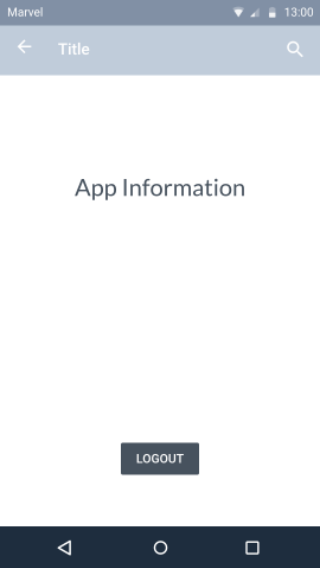
\includegraphics[scale=0.6]{design-options}
\end{center}

\newpage
\subsection{Create Chat Screen}
\begin{center}
    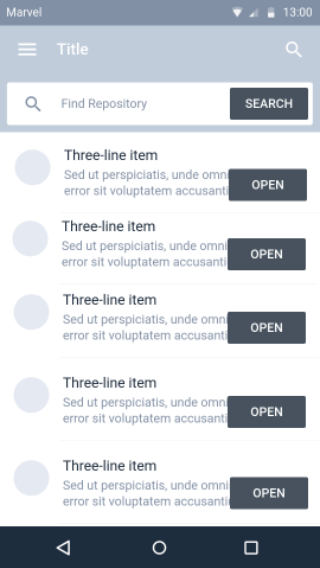
\includegraphics[scale=0.6]{design-create-chat}
\end{center}

\newpage
\subsection{Chat Screen}
\begin{center}
    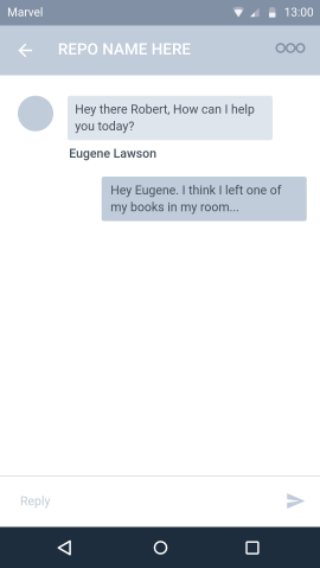
\includegraphics[scale=0.6]{design-chat}
\end{center}

\newpage
\subsection{Chat Info Screen}
\begin{center}
    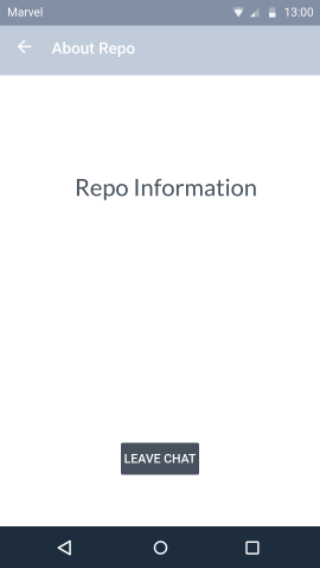
\includegraphics[scale=0.6]{design-chat-info}
\end{center}

\newpage
\section{User Story Coverage}

\begin{center}
    \begin{tabular}{ | p{0.9\linewidth} |}
        \hline
        \textbf{Login Screen} \begin{itemize}
            \item As a user, I can sign in with my GitHub account to sign into the app
        \end{itemize}\\
        \hline
        \textbf{Home Screen} \begin{itemize}
            \item As a user, I can view a list of recent chat rooms to quickly get back to what I was working on
            \item As a user, I can tap a star on a chat room to pin it ot the top of the list so I can keep chat rooms I want to keep on top
            \item As a user, I can select a chat room to open it up
        \end{itemize}\\
        \hline
        \textbf{Create Chat Screen}\begin{itemize}
            \item As a user, I can create a new chat room for a repository that I own so I can coordinate with other contributors
        \end{itemize}\\
        \hline
        \textbf{Chat Screen}\begin{itemize}
            \item As a user
        \end{itemize}\\
        \hline
        \textbf{Chat Info Screen}\begin{itemize}
            \item As a user
        \end{itemize}\\
        \hline
        \textbf{Options Screen}\begin{itemize}
            \item As a user
        \end{itemize}\\
        \hline
    \end{tabular}
\end{center}

\chapter{System Design}

\chapter{Iteration Planning}

\appendix
\chapter{Resources}

\begin{itemize}
    \item Microsoft Whiteboard
    \item Marvelapp.com
    \item \LaTeX
\end{itemize}

\end{document}
